\section{Teorías del aprendizaje: Modelo Push}


La primera manifestación de las \gls{tic} en la educación se da como un
sustituto a los medios tradicionales. Los materiales didácticos son
responsabilidad de los profesores, imprentas y
academias\cite{leinonen:ict,white:ict}.

El modelo \textit{push} favorece a las corrientes pedagógicas instruccionismo y
conductismo. El instruccionismo utiliza a las \gls{tic} para resolver problemas
de distancia y de costo\cite{igi:instructionism,johnson2005instructionism},
mientras que el conductismo utiliza a las \gls{tic} como un medio para proveer
refuerzos positivos\cite{weegar2012comparison}.

\subsection{Instruccionismo}

La educación tradicional o instruccionismo se basa en la transferencia de
conocimiento del profesor al alumno, se enfoca más en el profesor, en la
capacidad del mismo, y en el producto final como resultado de un proceso no
interactivo y bien
documentado\cite{igi:instructionism,johnson2005instructionism}. Los mecanismos
tradicionales para probar la efectividad de este tipo de enseñanza son los
exámenes escritos.

El instruccionismo es conocido además como enseñanza sistemática, enseñanza
explícita, enseñanza directa, y enseñanza
activa\cite{johnson2005instructionism}. Siempre se enfatiza en el
profesor\cite{johnson2005instructionism}.

Epistemológicamente se puede observar al instruccionismo como objetivo, pues
considera que el conocimiento es independiente del entorno, se asume que el
mismo es isomorfo, si el profesor puede enseñar, el alumno puede
aprender\cite{johnson2005instructionism}.

En el instruccionismo, la utilización de las \Gls{tic} se centra principalmente
en mecanismos para proveer contenido, se utilizan plataformas que
permiten a los profesores distribuir contenido y otras actividades relacionadas.

\subsubsection{Ejemplos}

Las aplicaciones de las \gls{tic} en el instruccionismo son:

\begin{itemize}

\item \textbf{E-Learning}: El \emph{E-Learning} se define como la educación y
    capacitación a través de medios digitales, incluye todo tipo de medio capaz
    de distribuir información, puede ser en tiempo real como salas de
    conversaciones y videoconferencias o puede ser diferido, como por ejemplo
    foros y enciclopedias\cite{punie:ict}.

    Una de las desventajas del \emph{e-Learning} es que se distribuye contenido
    masivamente a los alumnos, y luego, de manera discreta se permite a los
    mismos colaborar, dejando siempre en claro que primero se debe asimilar toda
    la información posible y luego relacionarse con los
    demás\cite{leinonen:ict}, es decir, los alumnos no forman parte de la
    creación del conocimiento.

    \begin{figure}[h] 
    \centering 
    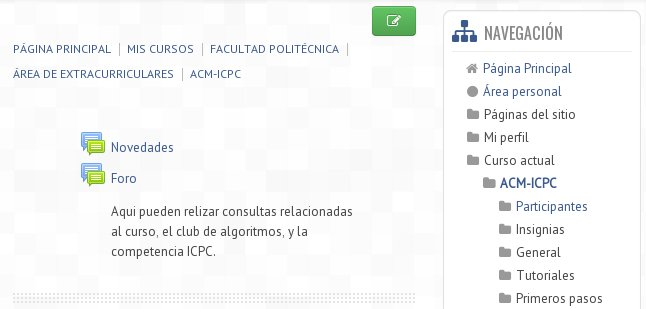
\includegraphics[scale=0.5]{tics/images/moodle.jpg}
    \caption{Moodle, plataforma de e Learning}\label{fig:moodle}
    \end{figure}

    La plataforma \emph{Moodle} (ver figura~\ref{fig:moodle}) cuya primera
    versión salió en el $2002$, es una de las principales herramientas del
    \emph{e-Learning} hoy en día, permite la creación de cursos específicos por
    materia y sitios especializados por instituciones
    académicas\cite{perkins2006using}. 

\item \textbf{Sustituto de medios tradicionales}: la utilización de las
    \gls{tic} desde sus inicios es como sustituto de los medios físicos, como
    libros y diapositivas por sus versiones digitales\cite{tinio:ict}.

\item \textbf{Clases a distancia}: las clases por videoconferencias y clases
    grabadas en video son herramientas utilizadas en reemplazo de las clases
    tradicionales. Permiten eliminar las distancias de tiempo y
    espacio\cite{tinio:ict}.

\end{itemize}

\subsection{Conductismo}

El conductismo es una corriente de la psicología, creada por \textit{Jhon
    Watson}, y posteriormente perfeccionada por \textit{Pavlov},
\textit{Skinner}, y \textit{Thorndik}. El conductismo defiende la idea de que
todas las acciones que realizan los seres vivos son consecuencia de un
estímulo\cite{weegar2012comparison}.

La primera utilización del conductismo con las \Gls{tic} es presentada por
\textit{Skinner}, en $1958$\cite{weegar2012comparison}, donde se describe una
máquina que contiene botones y una pantalla donde se presenta una pregunta, para
responder, el usuario dispone de varias opciones, cada opción esta relacionada
con un botón, si el aprendiz no presiona el botón correcto, debe seguir
intentando hasta responder correctamente y así
poder avanzar\cite{weegar2012comparison}, este es el inicio de lo que se conoce como
\enquote{Prueba y Error}.

Una característica del conductismo, es la ley de \textit{Thorndike}, la cual
indica que una acción, cuya consecuencia es un estímulo favorable, es más
probable que sea repetida\cite{weegar2012comparison}.

%A finales de la década de $1970$ e inicios de la década de $1980$,  la
%complejidad técnica de las computadoras limitaba la cantidad de herramientas
%disponibles, los programas eran desarrollados por profesores, y su objetivo era
%que los alumnos puedan poner en práctica lo aprendido en el aula. 

%\textbf{Aprendizaje como anexo:} el principal objetivo del desarrollo de un
%\emph{edutainment} es el de entretener, los objetivos pedagógicos son agregados
%al final. Adicionalmente, este aprendizaje se provee a través de largos textos
%que normalmente son omitidos.

\subsubsection{Ejemplos}
\label{sec:edutainment}

Entre los ejemplos de aplicación del conductismo en las \gls{tic} se encuentran:

\begin{itemize}

\item \textbf{Ejercicios de prueba y error}: son ejercicios en los cuales se
    presenta una pregunta y una lista de respuestas al alumno, y este debe
    responder correctamente. Si el alumno no responde correctamente, se repite
    la pregunta\cite{weegar2012comparison}.

\item \textbf{Edutainment}: son juegos sencillos que transmiten información
    simple al usuario, su estructura se basa en un objetivo claro que está
    separado de la experiencia educativa\cite{egenfeldt2007third}. El
    \emph{edutainment} pretende agregar entretenimiento a la educación, se ve al
    alumno como un receptor pasivo de información que debe asimilarla, y para
    aumentar la implicación de los alumnos, el entretenimiento es
    agregado\cite{resnick:2004}. Los \emph{edutainment} son el primer intento de
    unir el entretenimiento y la educación dentro de las
    \gls{tic}\cite{leinonen:ict}.

    Entre ejemplos de los \emph{edutainment}, podemos encontrar a:

    \begin{itemize}

    \item \textbf{Math Blaster}: (ver figura~\ref{fig:math_blaster}) es un
        \emph{edutainment} donde el alumno debe responder repetitivamente
        preguntas aritméticas para obtener municiones, luego con esas municiones
        debe completar diferentes misiones en una nave\cite{bruckman1999can}.
        Como todas las preguntas se responden mediante un mecanismo de selección
        múltiple, y no existe penalización por respuestas incorrectas, los
        alumnos no reflexionan sobre las respuestas elegidas, seleccionan una
        opción aleatoria y si no es la correcta, prueban otra, tras una cantidad
        finita de intentos, siempre se obtiene la recompensa deseada.

        \begin{figure}[H] 
        \centering 
        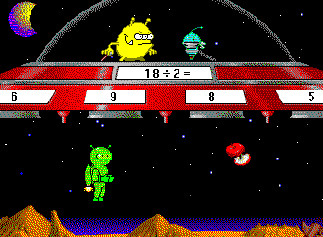
\includegraphics[scale=0.4]{tics/images/math_blaster.jpg}
        \caption{Math Blaster, \emph{edutainment} del año 1987}\label{fig:math_blaster} 
        \end{figure}

    \item \textbf{Donde en el mundo esta Carmen Sandiego} (ver
        figura~\ref{fig:carmen}) el objetivo del juego es detener a una serie de
        criminales mediante indicios que son proveídos en forma de texto. Este
        exitoso juego demuestra las falencias del \textit{Edutainment}, siendo
        visualmente muy atractivo, y con contenido multimedia acorde a su
        tiempo, no era más que \enquote{Prueba y Error}, cada nivel del juego
        podía ser completado sin leer la información
        proveída\cite{charsky:2010}.

        \begin{figure}[ht!] 
        \centering 
        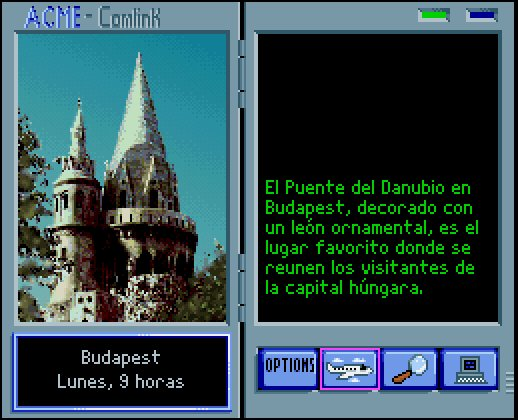
\includegraphics[scale=0.5]{tics/images/carmen.jpg}
        \caption{Donde en el mundo esta Carmen Sandiego}\label{fig:carmen}
        \end{figure}

    \end{itemize}

    Las aplicaciones se limitaban a matemáticas, lenguaje y geografía, donde se
    podía evaluar inmediatamente los resultados proveídos por los alumnos, pues,
    normalmente era un enunciado y una lista posible de opciones del tipo
    \enquote{Prueba y Error}\cite{leinonen:ict}. 

\end{itemize}

\subsection{Ventajas y desventajas del modelo Push}

Las ventajas del modelo \textit{push} son:

\begin{itemize}

\item Permite controlar el entorno del aprendizaje utilizando un enfoque
    científico. Se controla el entorno de los alumnos, los estímulos que recibe
    y las consecuencias de estos estímulos. Se ignora a los pensamientos y
    experiencias previas de las personas\cite{weegar2012comparison}.

\item Permite educar a personas con desafíos de aprendizaje y
    comportamiento\cite{johnson2005instructionism}.

\item Permite la enseñanza de pensamiento de bajo nivel\footnote{El pensamiento
        de bajo nivel está relacionado con las prácticas educacionales que
        incluyen la capacidad de memorizar y procesar, al contrario, el
        pensamiento de alto nivel incluye la capacidad de crear y
        evaluar\cite{edwards2000higher}}. Son excelentes para enseñar matemática
    básica, geografía y lenguaje\cite{charsky:2010}.

\end{itemize}

Las desventajas que presentan las corrientes del tipo \textit{push} son:

\begin{itemize}

\item No tienen en cuenta la experiencia previa de los alumnos ni el factor
    social. Los medios utilizados para la educación se centran en el profesor y
    en la manera de dar la clase\cite{siemens2008learning,sawyer2005cambridge}.

    El comportamiento humano no puede ser reducido, no solo responde a los
    estímulos y al entorno, sino, además responde a la experiencia
    previa\cite{weegar2012comparison}.

\item No se enfoca en los alumnos, no todos los alumnos aprenden al mismo
    nivel\cite{johnson2005instructionism}.

\item Desde el aspecto pedagógico, los alumnos tienen problemas para comprender
    ideas diferentes a las encontradas en clase\cite{sawyer2005cambridge}.

\item Los alumnos tienden a memorizar contenido sin entender el contexto en el
    cual fue creado el conocimiento\cite{sawyer2005cambridge}. 
    
\item Los alumnos tratan a los hechos y procedimientos como conocimiento
    estático, que no puede ser transformado, y que siempre es
    verdad\cite{sawyer2005cambridge}.

\item Se centra en motivaciones externas, y deja de lado la motivación interna.
    Las motivaciones externas son las recompensas que reciben los alumnos al
    llevar a cabo un ejercicio de manera correcta. La motivación interna es de
    gran importancia\cite{weegar2012comparison}.
    
\item Prueba y error, las aplicaciones creadas utilizando estas corrientes
    permiten al alumno intentar varias veces sin ser penalizados, además de que
    los alumnos no están motivados, provocan que el alumno pruebe las opciones
    sin el proceso de reflexión necesario para aprender. Es decir, se enseñaba a
    probar opciones sin sentido antes que entender y analizar la
    experiencia\cite{charsky:2010,egenfeldt2007third,bruckman1999can}.

\end{itemize}
